\documentclass{beamer}


%\beamertemplateshadingbackground{yellow!100}{white}
\usepackage[bulgarian]{babel}
\usepackage{amsfonts,amsmath}
\usepackage{graphicx}
\usepackage{sansmathaccent}
\pdfmapfile{+sansmathaccent.map}
\usepackage{multirow}
%\usetheme{Warsaw}
\usetheme[secheader]{Madrid}

\usepackage{multimedia}
\logo{
\includegraphics[height=0.5cm]{imi.jpg}}

\newcommand{\be}{\begin{equation}}
\newcommand{\ee}{\end{equation}}
\newcommand{\rf}[1]{(\ref{#1})}
\newcommand{\RR}{\mathbb{R}}
\newtheorem{thm}{Theorem}
\newtheorem{lm}{Lemma}

%\def\ra#1\{\renewcommand{\arraystretch}{#1}
\begin{document}
 %[propagating wave solutions to the 2D BPE]
\title{Числено решение на двумерното Парадигматично уравнение на Бусинеск}

\author{докторант: Красимир Ангелов 
\newline \newline научен ръководител: Наталия Кольковска}
\institute[IMI -- BAS]{Институт по Информатика и Математика\\ Българска Академия на Науките, София, България,\\ e-mail: angelow@math.bas.bg}

%================== frame 01 ======================================
\begin{frame}
\titlepage
\end{frame}

%---------- frame 02 ----------------
\begin{frame}
\tableofcontents 
\setbeamertemplate{table of contents shaded}[default]
\section{Преглед на литературата}
\section{Цели}
\section{Парадигматичното уравнение на Бусинеск - смяна на променливите}
\section{Числени методи за Парадигматичното уравнение на Бусинеск}
\subsection{Консервативна схема}
\subsubsection{Сходимост}
\subsubsection{Запазване на дискретната енергия}
\subsection{Метод на Тейлор и метод на правите}
\subsubsection{Сходимост}
\section{Числени резултати}
\subsection{Дискретните маса и енергия - сравнение между метода на Тейлор и Консервативната схема}
\subsection{Форма и максимум на решението при метода на Тейлор}
\subsection{Числен тест при $\beta = 3, c=0.3$}


%\tableofcontents 
\end{frame}

%---------- frame 03 ----------------
\begin{frame}
\frametitle{Преглед на литературата}

\begin{itemize}
  \item 2010, Christov, C.I., Kolkovska, N., Vasileva, D., On the Numerical Simulation of Un-
steady Solutions for the 2D BPE, {\it In: Numerical Methods and Applications},

  \item 2011, Chertok, A., Christov, C.I., Kurganov, A., Central-Upwind Schemes for the BPEs,
{\it Computational Science and High Performance Computing IV},

  \item 2012, Kolkovska, N., Angelow K., A Multicomponent Alternating Direction Method for Numerical Solving of Boussinesq Paradigm Equation, {\it In:  I. Dimov, I., Farago, I., Vulkov, L. (eds.) NAA},
  
  \item 2013, Dimova M., Vasileva D., Comparison of Two Numerical Approaches to Boussinesq Paradigm Equation,  {\it Lect. Notes Comput. Sci.}, 
  
  \item 2022, Yuyu He, Hongtao Chen, Efficient algorithm and convergence analysis of conservative SAV compact difference scheme for Boussinesq Paradigm equation, {\it Computers and Mathematics with Applications}
\end{itemize}

\end{frame}

%---------- frame 04 ----------------

\begin{frame}
\frametitle{Цели}

\begin{itemize}
  \item да се построи числен метод (на Тейлор), който използва диференчни схеми с висок (втори, четвърти и шести) ред на апроксимация, за решението на Парадигматичното уравнение на Бусинеск,
  
  \item да се приложи нов тип начално условие, което е намерено числено (понеже не съществува явна формула) и апроксимацията му отговаря на апроксимацията използвана в метода на Тейлор,
  
    \item да се изследва Парадигматичното уравнение на Бусинеск при по-високи скорости близки до допустимия максимум $c \approx \min (1/ \sqrt{\beta_1},1)$, $c < \min (1/ \sqrt{\beta_1},1)$, използвайки гореспоменатото начално условие,

  \item да се сравнят числените резултати получени с метода на Тейлор и Консервативната схема при втори ред на апроксимация,

  \item да се изследват измененията в максимума и формата на численото решение в зависимост от реда на апроксимация,
    
\end{itemize}


\end{frame}

%---------- frame 05 ----------------

\begin{frame}
\frametitle{Публикации}

Резултатите от численото решение на двумерните стационарно и хиперболични уравнения на Бусинеск са
публикувани в
\begin{itemize}
  \item K. Angelow, N. Kolkovska, Numerical Study of Traveling Wave Solutions to 2D BE, {\it Serdica Journal of Computing},
  \item K. Angelow, New Boundary Condition for the Two Dimensional Stationary Boussinesq Paradigm Equation, {\it International Journal of Applied Mathematics},
   \item K. Angelow, Comparison Between Two Numerical Methods for Solution of 2D BPE, {\it AIP Conference Proceedings}
\end{itemize}

\end{frame}
%---------- frame 06 ----------------

\begin{frame}
\frametitle{Boussinesq Paradigm Equation}

The goal of this talk is to:
\begin{itemize}
 \item propose numerical method with high approximation order for the solution of BPE,
 \item investigate properties of the resulting waves for velocities, which are close to the maximum $c \approx c_{max}$, $c < c_{max}$:
	\begin{itemize}
	 \item energy,
	 \item shape,
	 \item maximum,
	\end{itemize}
\end{itemize}
where $c_{max} = min\{1, \sqrt{ \frac{\beta_2}{\beta_1} } \}$.
\end{frame}


%---------- frame 07 ----------------

\begin{frame}
\frametitle{Boussinesq Paradigm Equation}
The following variable change
\begin{align}
x = \sqrt{\beta_1} \bar{x}, \quad y = \sqrt{\beta_1} \bar{y}, \quad t = \sqrt{\beta_1} \bar{t}
\end{align}

transforms (1) into 

\be\label{problemVC}
\beta(I-\Delta) \frac{\partial^2 u}{\partial t^2}=
  \Delta u -\Delta^2 u +\Delta(-\alpha \beta u^2 + (\beta - 1 )u)
\ee

where $\beta = \beta_1/\beta_2$.

\end{frame}



%---------- frame 05 ----------------
\begin{frame}
\frametitle{Conservation of the Energy}
The mass:

\begin{equation}\label{int}
D(u(t))=D(u(0))=\int_{R^2} u(x,y)dx dy
\end{equation}

and energy:
\begin{align}\label{ex-en}
E(u(t)) = E(u(0)) =&\int_{R^2} u_t \left((A^{-1}+E)u_t\right) dxdy+
\beta \int_{R^2} u^2 dxdy \nonumber\\
+& \int_{R^2}u \left(A u\right) dxdy
-\frac{2 \alpha \beta}{3} \int_{R^2} u^3 dxdy =const
\end{align}
of the continuous problem \rf{problemVC}. Here $E(u)$ is the exact energy of problem \rf{problemVC} and $Au=-\Delta u$.
\end{frame}

%-----------------------------------------------------------------

\begin{frame}
\frametitle{The Computational Domain $\Omega_h$}
\framesubtitle{Equidistant Grid $h=(h_1, h_2)$}
\begin{center}\vspace{0.4cm}
	\begin{minipage}[b]{0.6\linewidth}
		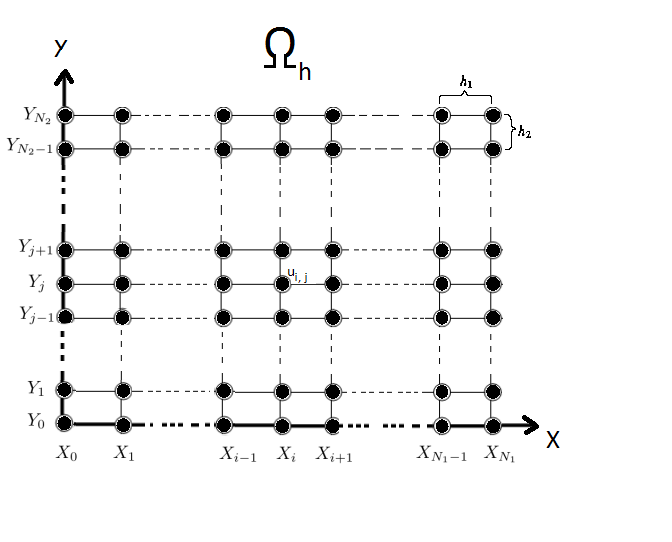
\includegraphics[width=\linewidth]{Omega_dah.png}
	\end{minipage}
\end{center}

\end{frame}

%---------- frame ----------------

\begin{frame}
\frametitle{Conservative FDS}
The approximation of the differential operators is defined as:
\begin{equation}
\frac{\partial^2 u}{\partial t^2}(x_i, y_j, t_k ) = \frac{ u^{(k+1)}_{i, j} - 2u^{(k)}_{i,j} + u^{(k-1)}_{i,j} }{\tau^2} + O(\tau^2) 
\end{equation}

\begin{equation}
\frac{\partial^2 u}{\partial x^2}(x_i, y_j, t_k ) = \frac{ u^{(k)}_{i+1, j} - 2u^{(k)}_{i,j} + u^{(k)}_{i-1,j} }{h_1^2} + O(h_1^2) 
\end{equation}

\begin{equation}
\frac{\partial^2 u}{\partial y^2}(x_i, y_j, t_k ) = \frac{ u^{(k)}_{i, j+1} - 2u^{(k)}_{i,j} + u^{(k)}_{i,j-1} }{h_2^2} + O(h_2^2) 
\end{equation}


\begin{equation}
\Delta_h u(x_i, y_j, t_k )  = \frac{ u^{(k)}_{i+1, j} - 2u^{(k)}_{i,j} + u^{(k)}_{i-1,j} }{h_1^2} + \frac{ u^{(k)}_{i, j+1} - 2u^{(k)}_{i,j} + u^{(k)}_{i,j-1} }{h_2^2}
\end{equation}

\end{frame}

%------------------------------------------------------------------

\begin{frame}
\frametitle{Conservative FDS}
The grid function obtained from [\ref{problemVC}] is defined as:
\begin{equation}
\beta (I-\Delta_h)\frac{ u^{(k+1)}_{i, j} - 2u^{(k)}_{i,j} + u^{(k-1)}_{i,j} }{\tau^2} = (\Delta_h - \Delta_h^2)u^{(k)}_{i,j} + \Delta_h(g(u^{(k)}_{i,j}))
\end{equation}
%
where the non-linear term $g$ is defined as:
\begin{align}
g(u^{(k)}_{i,j})=& -\frac{\alpha \beta} { 3 } \left( (u^{(k+1)}_{i,j})^2 + (u^{(k-1)}_{i,j})(u^{(k+1)}_{i,j}) + (u^{(k-1)}_{i,j})^2 \right) + \nonumber\\
+&\frac{ (\beta - 1 )}{ 2 }\left( u^{(k+1)}_{i,j} + u^{(k-1)}_{i,j} \right).
\end{align}


\end{frame}


%------------------------------------------------------------------

\begin{frame}
\frametitle{TS Approach with Method of Lines}
\begin{center}\vspace{0.25cm}
	\begin{minipage}[b]{0.45\linewidth}
		 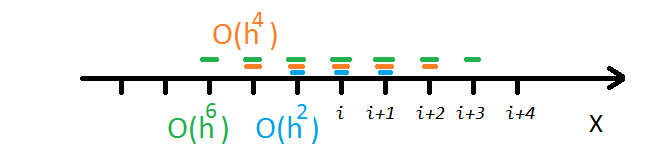
\includegraphics[width=\linewidth]{../amitans/figures/FDS.png}
	\end{minipage}	
\end{center}
Let $\Delta_h u_{i,j}$ be the approximation of $\Delta u$ with $O(|h|^2)$, $O(|h|^4)$, $O(|h|^6)$.
\\
Let $u_{i,j}(t)$ be the approximation of $u(x_i, y_j, t)$ at grid point $(x_i, y_j)$.
\\
%here99
From [\ref{problemVC}] one obtains a system of ODEs:
\be \label{DiscreteEq}
\beta (I-\Delta_h) \frac{\partial^2 u}{\partial t^2}(x_i, y_j, t)=
 (\Delta_h - \Delta_h^2) u_{i, j}(t) + \Delta_h ( g( u_{i, j}(t) ) )
\ee
for $i = 0..N_1$ and $j=0..N_2$. For each ODE in the system we do TS expansion:
\begin{align} \label{TSe}
u(x_i, y_j, t+\tau) = u(x_i, y_j, t) + \tau \frac{ \partial u }{ \partial t }(x_i, y_j, t)  + ... 
%\nonumber
%\\
\frac{ \tau^p }{ p! } \frac{ \partial^p u }{ \partial t^p }(x_i, y_j, t) + O(\tau^{p+1})
\end{align}
for some natural number $p \ge 2$.
\end{frame}

%------------------------------------------------------------------

\begin{frame}
\frametitle{TS Approach with Method of Lines}
Evaluating formula [\ref{TSe}]
\begin{itemize}
 \item IC $\rightarrow$ $u(x_i, y_j, t=0)$, $\frac{ \partial u }{ \partial t }(x_i, y_j, t=0)$,
 \item $[$\ref{DiscreteEq}$]$ $\rightarrow$ $\frac{ \partial^2 u }{ \partial t^2 }(x_i, y_j, t=0)$ ,
 \item Differentiating equation $\frac{ \partial^{p-2} u }{ \partial t^{p-2} }$ [\ref{DiscreteEq}] $\rightarrow$  $\frac{ \partial^p u }{ \partial t^p }(x_i, y_j, t)$,
 \item Substitute the evaluated derivatives in formula $[$ \ref{TSe} $]$.
\end{itemize}


Thus one gets the following approximations
\begin{description}
 \item[$p=2$] $O(|h|^2 + \tau^2)$,
 \item[$p=4$] $O(|h|^4 + \tau^4)$,
 \item[$p=6$] $O(|h|^6 + \tau^6)$.
\end{description}
%The complexity of the algorithm is
%$$ O( N_1 N_2 N_3 p ) $$
%where $N_1 N_2$ is the number of points in $\Omega_h$ and $N_3 = T/\tau$.
\end{frame}

%------------------------------------------------------------------

\begin{frame}
\frametitle{Validation and Results}
Two parameters sets are used:
\begin{description}
 \item[Test 1] $\beta = 3$, $c = 0.45$, $\Omega = [-30, 30] \times [-27, 27]$, $T = 10$
 \item[Test 2] $\beta = 1$, $c = 0.9$, $\Omega = [-128, 128] \times [-58, 58]$, $T = 10$
\end{description}

Numerical methods applied for each Test:
\begin{enumerate}
  \item Conservative FDS with $O(|h|^2 + \tau^2)$
  \item TS method with $O(|h|^p + \tau^p)$ and $p = 2, 4, 6$
\end{enumerate}

Test 1 and Test 2 use zero boundary condition, i.e. values of the finite difference stencil outside the numerical domain $\Omega_h$ are zeros.
\end{frame}

%------------------------------------------------------------------

\begin{frame}
%C
\frametitle{Convergence for Conservative FDS}
$T = 10$
\begin{table}[ht]
\centering
\small
		\begin{tabular}{||c|l|ll|ll||}
			\hline
			\hline
      \multirow{2  }{*}{FDS}        & \multirow{2  }{*}{$h$, $\tau$}  & \multirow{2  }{*}{errors $E_i$in$L_2$}  &Conv.& \multirow{2  }{*}{errors $E_i$in$L_\infty$}  &Conv.  \\
	                                        &                                                     &                                                                 &  Rate &                                                                       & Rate \\
   			\hline 
					\hline 
  $\beta=3$                &0.2, 0.001         &                    &                &                  &                   \\
   c=0.45                     &0.1, 0.0005         & 0.989422   &                & 1.043649  &                   \\
     $O(h^2 + \tau^ 2)$ &0.05, 0.00025  &0.344818    & 1.52       & 0.355517   &   1.55   \\
	   \hline
			\hline 
       $\beta=1$           & 0.4, 0.002       &                   &           &                 &   \\
                  c=0.9       & 0.2, 0.001        & 0.200424   &          &0.072726  &   \\
  $O(h^2+ \tau^2)$  & 0.1, 0.0005       & 0.047899   & 2.06  &0.021451  & 1.76 \\
	   \hline
			\hline 
		\end{tabular}
		\caption{Convergence tests for the Conservative FDS method with zero boundary and approximation errors $O(h^{2} + \tau^2 )$. Errors $E_i$ are measured in $L_2$ and $L_\infty$ norms}
\label{tableC}
\end{table}

\end{frame}


%------------------------------------------------------------------

\begin{frame}
\frametitle{Convergence for TS Approach}
%A
$T = 10$
\begin{table}[ht]
\centering
\small
\resizebox{0.6\linewidth}{!}{%
		\begin{tabular}{||c|l|ll|ll||}
			\hline
			\hline
      \multirow{2  }{*}{FDS}        & \multirow{2  }{*}{$h$, $\tau$}  & \multirow{2  }{*}{errors $E_i$in$L_2$}  &Conv.& \multirow{2  }{*}{errors $E_i$in$L_\infty$}  &Conv.  \\
	         &                    &                               & Rate   &                                        & Rate \\
   			\hline 
					\hline 
  $\beta=3$                &0.2, 0.001          &              &              &                     &      \\
   c=0.45                     &0.1, 0.0005          &0.989414 &            &1.043641    &       \\
     $O(h^2 + \tau^ 2)$ &0.05, 0.00025   & 0.344813 & 1.52    &0.355511    &  1.55      \\
			\hline 
  $\beta=3$               &0.2, 0.02       &              &            &                     &      \\
   c=0.45                    &0.1, 0.01      &0.191224 &            &0.193874    &       \\
     $O(h^4+ \tau^4)$ &0.05, 0.005&0.013029 & 3.87   &0.013656     &3.82       \\
			\hline 
  $\beta=3$               &0.2, 0.02       &                &            &                     &      \\
     c=0.45                 &0.1, 0.01        &0.032671 &            &  0.033626    &       \\
     $O(h^6+ \tau^6)$ &0.05, 0.005 &0.000598 &5.77     & 0.000635    & 5.72       \\
	   \hline
			\hline 
       $\beta=1$       &0.4, 0.002        &             &            &           &   \\
                  c=0.9    &0.2, 0.001       &  0.20366   &            &0.075854 &   \\
  $O(h^2+ \tau^2)$ &0.1, 0.0005   &0.048320   &2.07  &0.022307  & 1.77 \\
			\hline
      $\beta=1$               &0.4, 0.04    &            &               &             &    \\
       c=0.9                     &0.2, 0.02     & 0.028275   &        &  0.013518   &   \\
       $O(h^4+ \tau^4)$ &0.1, 0.01   &0.001812 & 3.96  & 0.000971  & 3.80  \\
    \hline
  $\beta=1$     &0.4, 0.04   &            &          &                  &      \\
      c=0.9                    &0.2, 0.02   &0.006734 &           & 0.003338      &       \\
     $O(h^6+ \tau^6)$ &0.1, 0.01 & 0.000232 &4.86 & 0.000069  & 5.60        \\
	   \hline
			\hline 
		\end{tabular}
		}%
		\caption{Convergence tests for Taylor method with zero boundary and different approximation errors $O(h^{2} + \tau^2 )$, $O(h^{4} + \tau^4 )$ and $O(h^{6} + \tau^6 )$. Errors $E_i$ are measured in $L_2$ and $L_\infty$ norms}
\label{table:A}
\end{table}

\end{frame}

%------------------------------------------------------------------

\begin{frame}
\frametitle{Results}
\framesubtitle{Energy for the Conservative scheme and TS method}

\begin{center}\vspace{0.4cm}
	\begin{minipage}[b]{0.49\linewidth}
		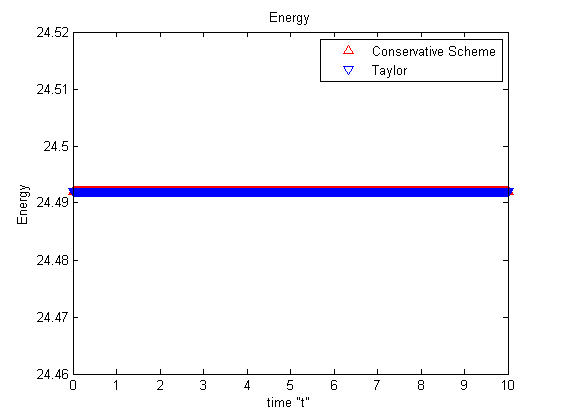
\includegraphics[width=\linewidth]{../amitans/figures/Energy_bt3_c045_h005.png}
	\end{minipage}	
	\begin{minipage}[b]{0.49\linewidth}
		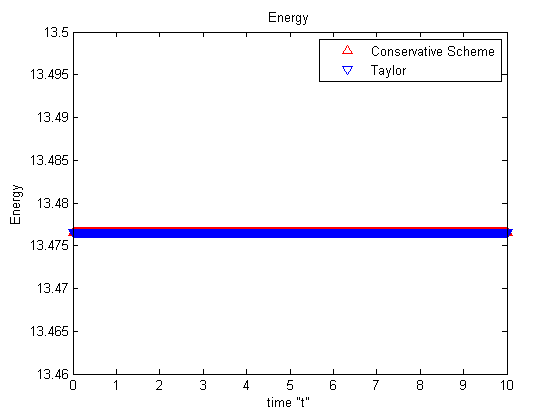
\includegraphics[width=\linewidth]{../amitans/figures/Energy_bt1_c090_h010.png}
		
	\end{minipage}
\end{center}
The Energy of the solution for approximation $O(|h|^2 + \tau^2)$ and $T = 10$. Left panel is for Test 1 with $\beta=3$, $c = 0.45$ and right panel is for Test 2 with $\beta=1$, $c = 0.9$.
\end{frame}




\begin{frame}
\frametitle{Results}
\framesubtitle{Wave Comparison}
\begin{center}\vspace{0.4cm}
	\begin{minipage}[b]{0.32\linewidth}
		 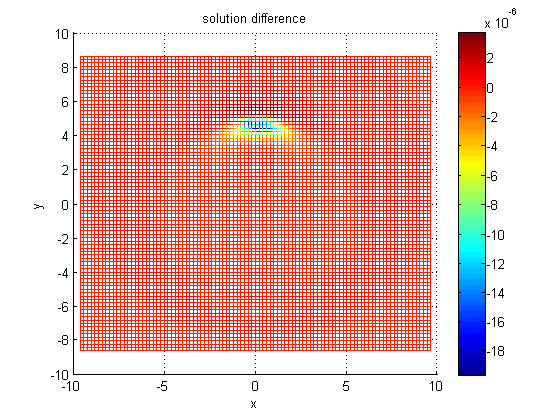
\includegraphics[width=\linewidth]{../amitans/figures/compare_30_bt3_c045_h020.png}
	\end{minipage}	
	\begin{minipage}[b]{0.32\linewidth}
		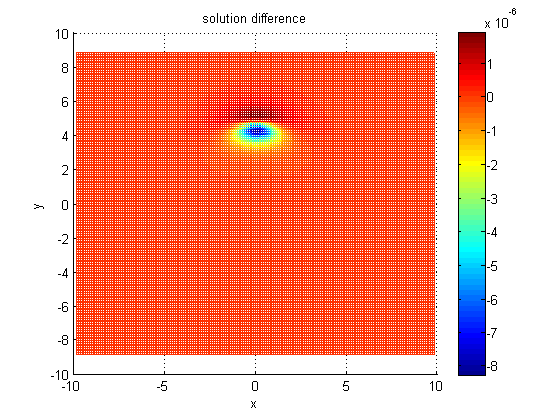
\includegraphics[width=\linewidth]{../amitans/figures/compare_30_bt3_c045_h010.png}
	\end{minipage}	
	\begin{minipage}[b]{0.32\linewidth}		
		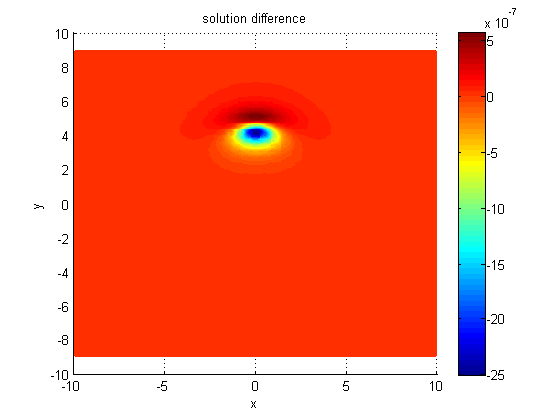
\includegraphics[width=\linewidth]{../amitans/figures/compare_30_bt3_c045_h005.png}
	\end{minipage}
\end{center}
Difference between solutions from TS approach and Conservative Scheme at time $T=10$, $O(|h|^2 + \tau^2)$ for Test 1. From Left to right $h=0.2, 0.1, 0.05$. The graphics represent only one nineth of the whole domain $\Omega_h$.
\end{frame}

%------------------------------------------------------------------

\begin{frame}
\frametitle{Results}
\framesubtitle{Wave Comparison}
\begin{center}\vspace{0.4cm}
	\begin{minipage}[b]{0.32\linewidth}
		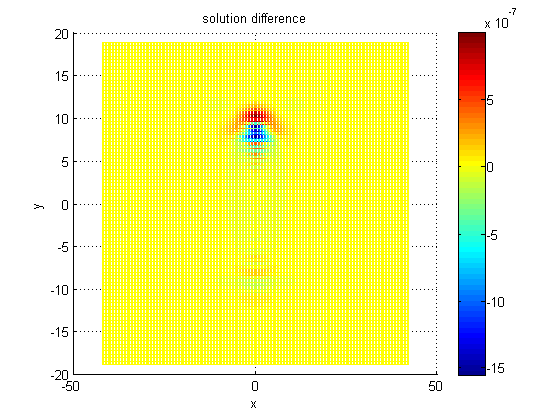
\includegraphics[width=\linewidth]{../amitans/figures/compare_128_bt1_c09_h040.png}
	\end{minipage}	
	\begin{minipage}[b]{0.32\linewidth}
		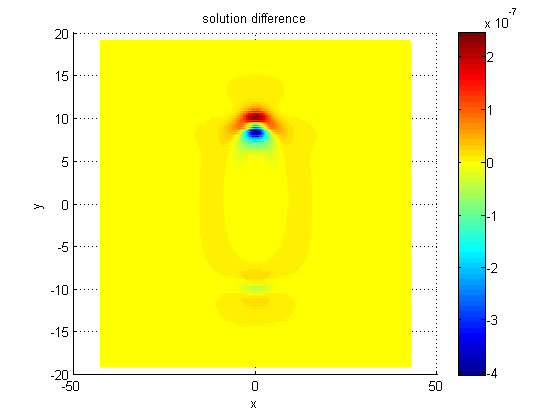
\includegraphics[width=\linewidth]{../amitans/figures/compare_128_bt1_c09_h020.png}
	\end{minipage}	
	\begin{minipage}[b]{0.32\linewidth}
		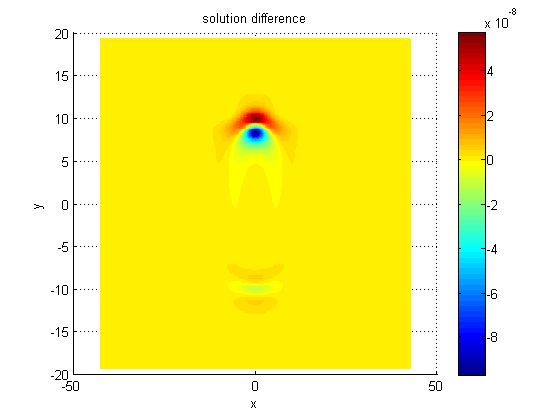
\includegraphics[width=\linewidth]{../amitans/figures/compare_128_bt1_c09_h010.png}		 
	\end{minipage}
\end{center}
Difference between solutions from TS approach and Conservative Scheme at time $T=10$, $O(|h|^2 + \tau^2)$ for Test 2. From Left to right $h=0.4, 0.2, 0.1$. The graphics represent only one nineth of the whole domain $\Omega_h$.
\end{frame}

%------------------------------------------------------------------

\begin{frame}
\frametitle{Results}
\framesubtitle{Solution Maximum, Taylor Series, smallest step sizes}

\begin{figure}[ht]
	\centering
	\begin{minipage}[b]{0.4\linewidth}
		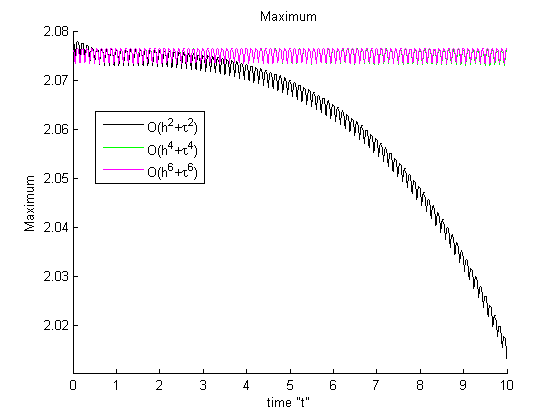
\includegraphics[width=\linewidth]{../amitans/figures/maximum_30_bt3_c045_h005.png}
	\end{minipage}	
	\begin{minipage}[b]{0.4\linewidth}
		 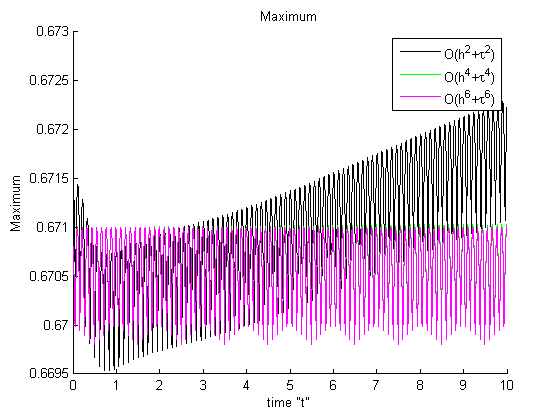
\includegraphics[width=\linewidth]{../amitans/figures/maximum_128_bt1_c090_h010.png}
	\end{minipage}

Evolution of the maximum for Test Wave 1 with $\beta =3$ (left panel) and Test Wave 2 with $\beta=1$ (right panel) for $T=10$.
\end{figure}

\end{frame}

%------------------------------------------------------------------

\begin{frame}
\frametitle{Results}
\framesubtitle{Solution Shape, Taylor Series, smallest step sizes, $O(|h|^6+\tau^6)$}
\begin{figure}[ht]
	\centering
	\begin{minipage}[b]{0.49\linewidth}
		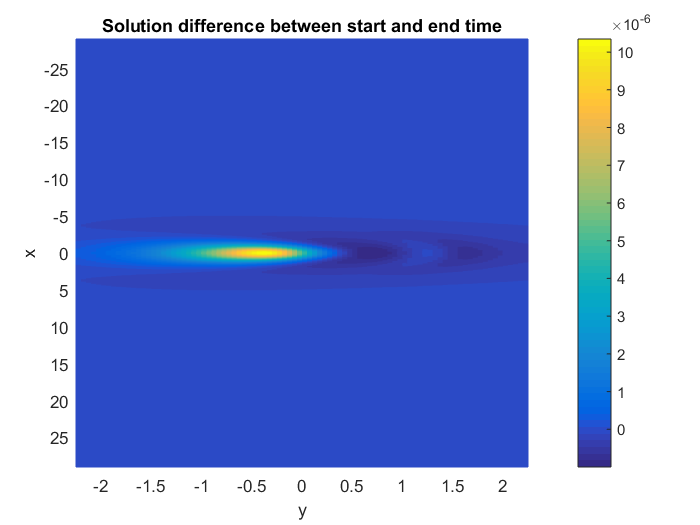
\includegraphics[width=\linewidth]{../amitans/figures/compare_start_end_bt3_c045_T10.png}
	\end{minipage}	
	\begin{minipage}[b]{0.49\linewidth}
		 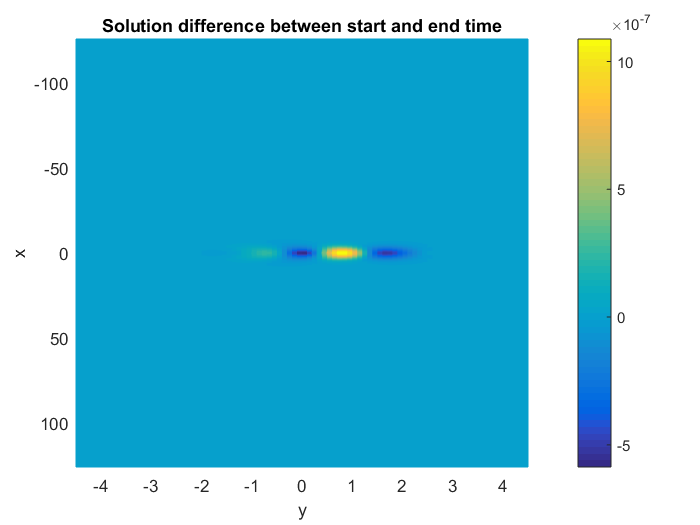
\includegraphics[width=\linewidth]{../amitans/figures/compare_start_end_bt1_c090_T10.png}
	\end{minipage}

Difference between localized wave at time $T=0$ and $T=10$ for Test Wave 1 with $\beta =3$  (left) and Test Wave 2 with $\beta=1$ (right). 
\end{figure}

It is obtained that:
\begin{description}
 \item[$\beta = 3$, $c = 0.45$] $||u_h(t=10)-u_h(t=0)|_{L_2} =  0.00000981$
 \item[$\beta = 1$, $c = 0.9$] $||u_h(t=10)-u_h(t=0)|_{L_2} = 0.00000186$
\end{description}
\end{frame}

%------------------------------------------------------------------

\begin{frame}
\frametitle{Conclusion}

\begin{description}
 \item[-] 2D BPE is solved using TS method with high approximation orders $O(|h|^k+\tau^k)$, $k=2,4,6$
 \item[-] the results are compared with the Conservative Scheme for $O(|h|^2+\tau^2)$
 \item[-] the Energy of the TS solution is saved with high accuracy over the time interval $[0, 10]$
 \item[-] the numerical solutions for wave speeds near the upper limit $c_{max} = min\{1, \sqrt{\beta_2/\beta_1} \}$ are stable in form and their maximums change with small errors over the time interval $[0, 10]$.
\item[-] the obtained solutions show soliton behavior!
\end{description}

\end{frame}

%------------------------------------------------------------------

\begin{frame}
\frametitle{Thank You For Your Attention!}
\framesubtitle{The Wave Evolution}
\begin{center}\vspace{0.4cm}
	\begin{minipage}[b]{0.30\linewidth}
		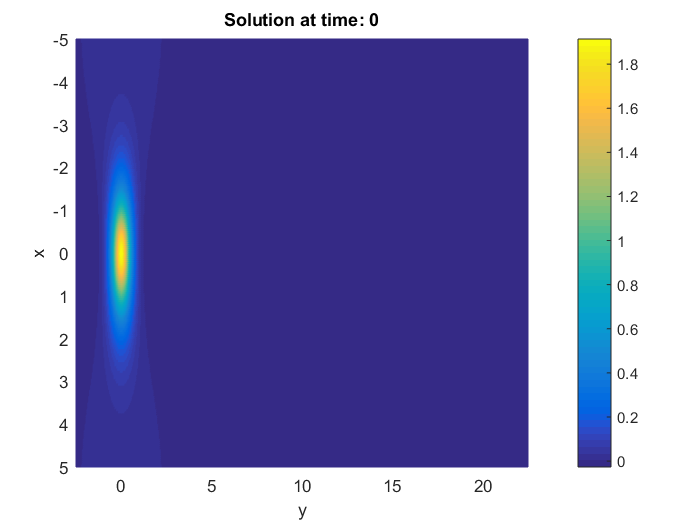
\includegraphics[width=\linewidth]{../amitans/figures/Solution_bt3_t=0.png}
	\end{minipage}	
	\begin{minipage}[b]{0.30\linewidth}
		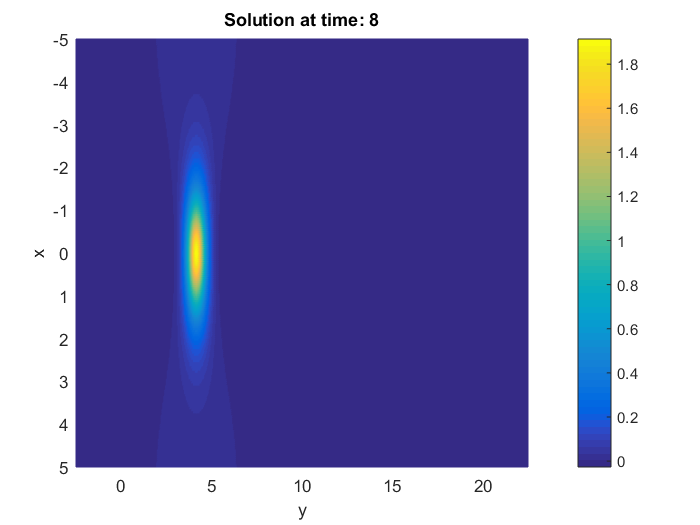
\includegraphics[width=\linewidth]{../amitans/figures/Solution_bt3_t=8.png}
	\end{minipage}	
	\begin{minipage}[b]{0.30\linewidth}
		 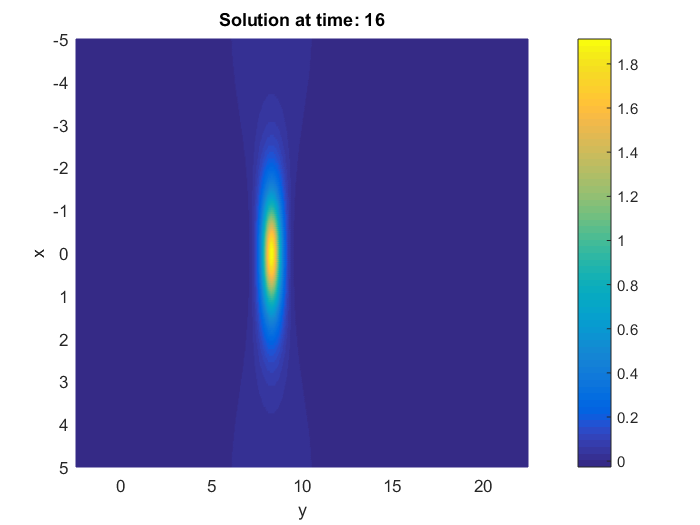
\includegraphics[width=\linewidth]{../amitans/figures/Solution_bt3_t=16.png}
	\end{minipage}
	\begin{minipage}[b]{0.30\linewidth}
		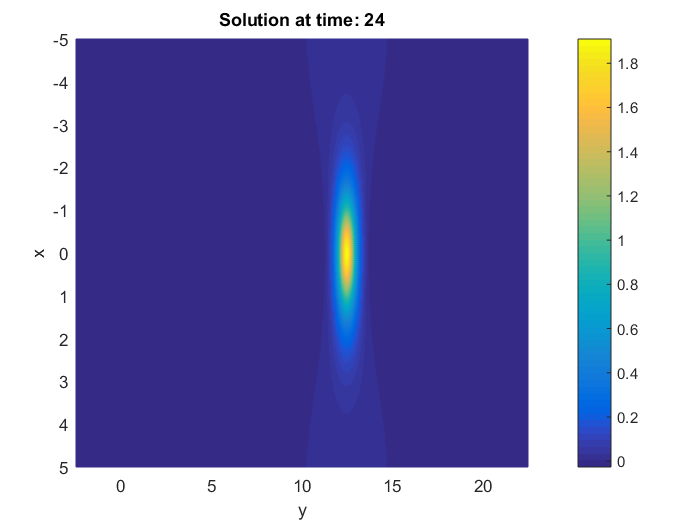
\includegraphics[width=\linewidth]{../amitans/figures/Solution_bt3_t=24.png}
	\end{minipage}	
	\begin{minipage}[b]{0.30\linewidth}
		 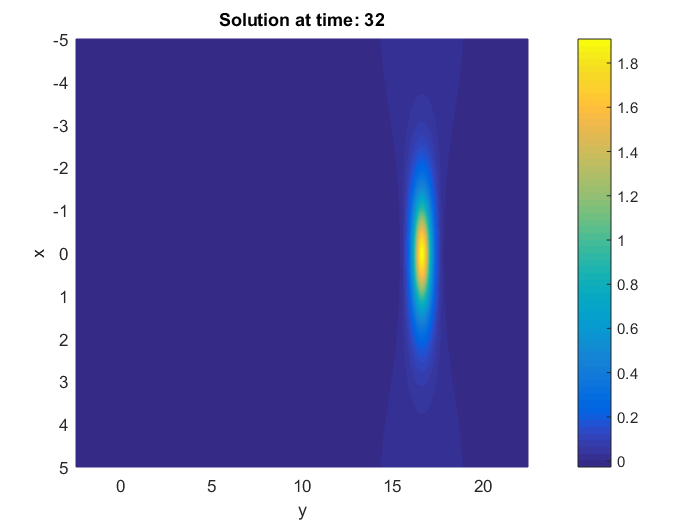
\includegraphics[width=\linewidth]{../amitans/figures/Solution_bt3_t=32.png}
	\end{minipage}
	\begin{minipage}[b]{0.30\linewidth}
		 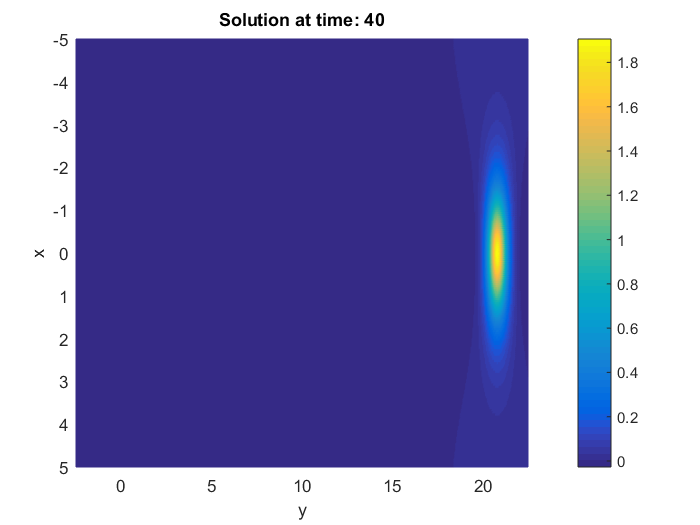
\includegraphics[width=\linewidth]{../amitans/figures/Solution_bt3_t=40.png}
	\end{minipage}
\end{center}
Numerical solution of single wave for $\beta=3$ and $c = 0.52$ at times $t=0,8,16,24,32,40$.
\end{frame}

%------------------------------------------------------------------

\begin{frame}
\frametitle{Wave Evolution}
\begin{center}\vspace{0.4cm}
	\begin{minipage}[b]{0.30\linewidth}
		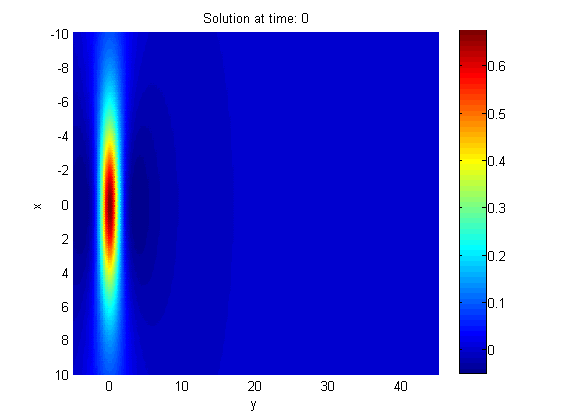
\includegraphics[width=\linewidth]{../amitans/figures/Solution1_t=0.png}
	\end{minipage}	
	\begin{minipage}[b]{0.30\linewidth}
		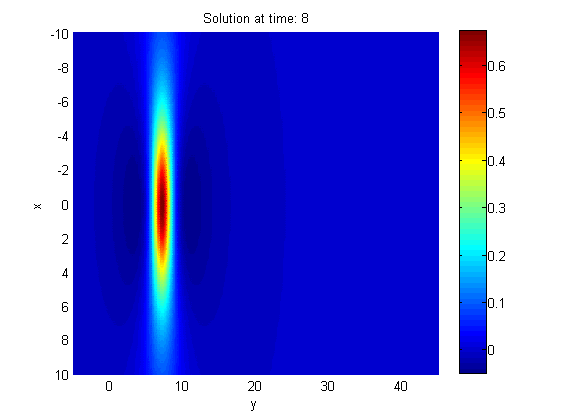
\includegraphics[width=\linewidth]{../amitans/figures/Solution1_t=8.png}
	\end{minipage}	
	\begin{minipage}[b]{0.30\linewidth}
		 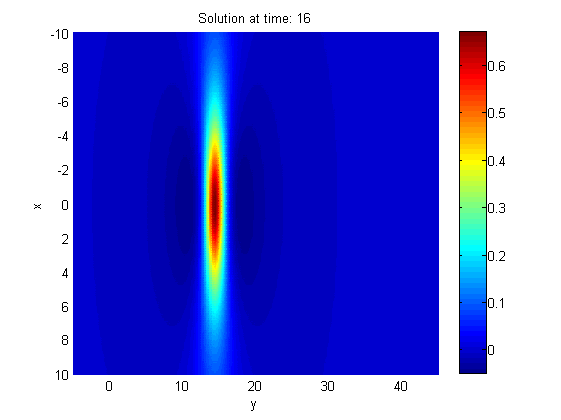
\includegraphics[width=\linewidth]{../amitans/figures/Solution1_t=16.png}
	\end{minipage}
	\begin{minipage}[b]{0.30\linewidth}
		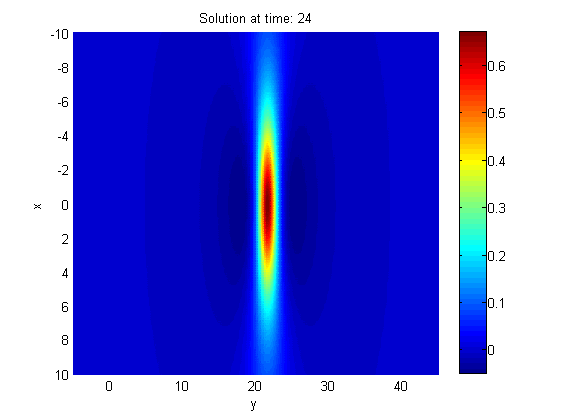
\includegraphics[width=\linewidth]{../amitans/figures/Solution1_t=24.png}
	\end{minipage}	
	\begin{minipage}[b]{0.30\linewidth}
		 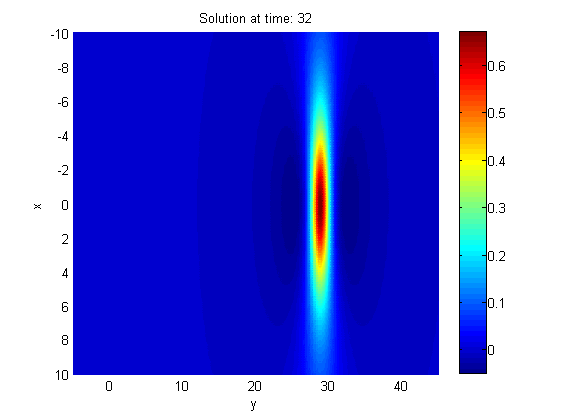
\includegraphics[width=\linewidth]{../amitans/figures/Solution1_t=32.png}
	\end{minipage}
	\begin{minipage}[b]{0.30\linewidth}
		 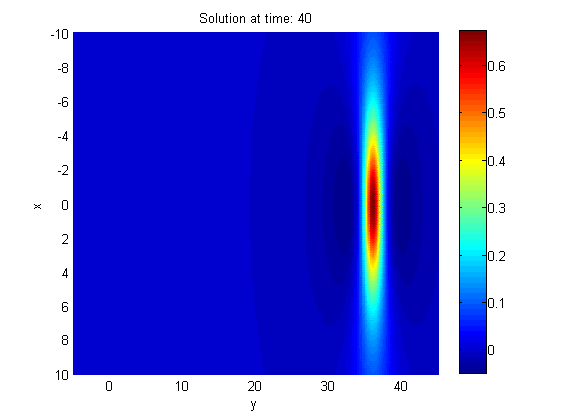
\includegraphics[width=\linewidth]{../amitans/figures/Solution1_t=40.png}
	\end{minipage}
\end{center}
Numerical solution of single wave for $\beta=1$ and $c = 0.9$ at times $t=0,8,16,24,32,40$.
\end{frame}

%------------------------------------------------------------------

\begin{frame}
\frametitle{Results}
\framesubtitle{Solution Maximum, Taylor Series, $O(|h|^6+\tau^6)$}

Two parameters sets are used:
\begin{description}
 \item[Test 3] $\beta = 3$, $c = 0.52$, $\Omega = [-40, 40] \times [-40, 60]$
 \item[Test 4] $\beta = 1$, $c = 0.9$, $\Omega = [-40, 40] \times [-80, 80]$
\end{description}
The end time is $T=40$ for both tests.
\begin{figure}[ht]
	\centering
	\begin{minipage}[b]{0.4\linewidth}
		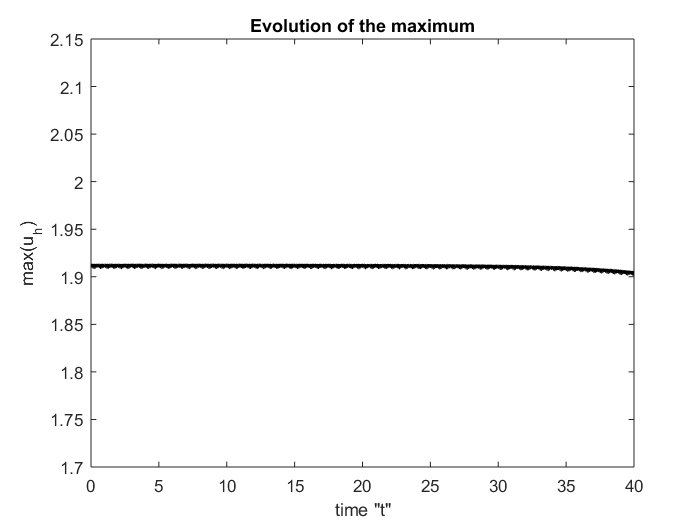
\includegraphics[width=\linewidth]{../amitans/figures/EvolutionOfMaximum_bt3_t40.png}
	\end{minipage}	
	\begin{minipage}[b]{0.4\linewidth}
		 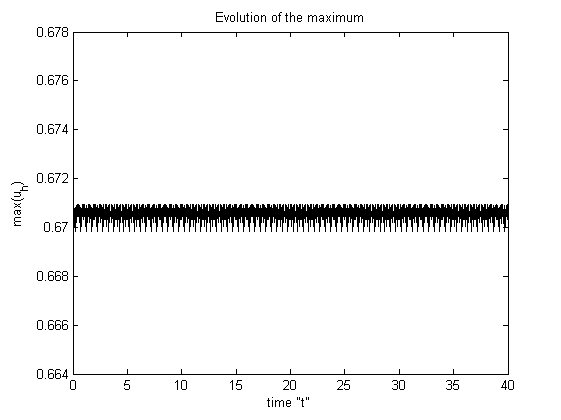
\includegraphics[width=\linewidth]{../amitans/figures/EvolutionOfMaximum_bt1_t40.png}
	\end{minipage}

Evolution of the maximum for Test Wave $\beta =3$ (left panel) and $\beta=1$ (right panel).
\end{figure}

\end{frame}

%------------------------------------------------------------------

\begin{frame}
\frametitle{Results}
\framesubtitle{Solution Shape, Taylor Series, $O(|h|^6+\tau^6)$}
\begin{figure}[ht]
	\centering
	\begin{minipage}[b]{0.49\linewidth}
		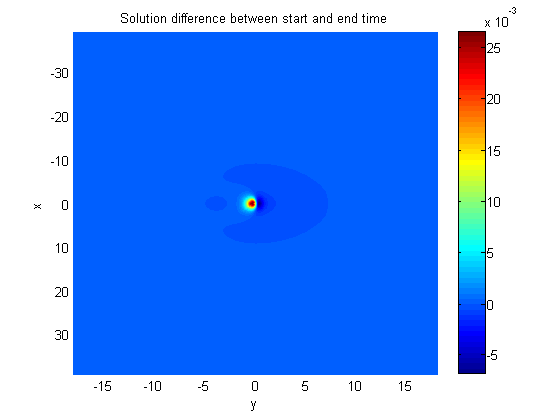
\includegraphics[width=\linewidth]{../amitans/figures/compare_start_end_bt3_c052.png}
	\end{minipage}	
	\begin{minipage}[b]{0.49\linewidth}
		 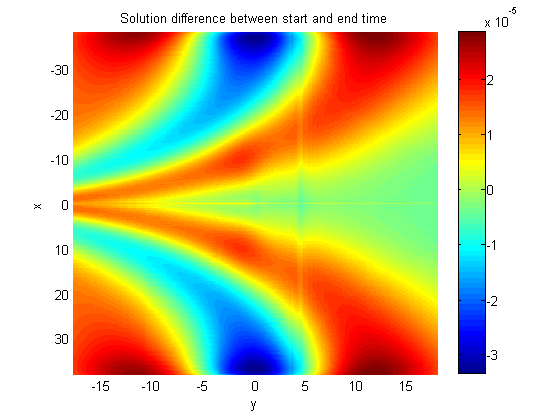
\includegraphics[width=\linewidth]{../amitans/figures/compare_start_end_bt1_c09.png}
	\end{minipage}

Difference between localized solitons at time $T=0$ and $T=40$ for Test 3 $\beta = 3$, $\beta = 0.52$  (left) and Test 4 $\beta=1$, $c=0.9$ (right). 
\end{figure}

It is obtained that:
\begin{description}
 \item[$\beta = 3$, $c = 0.52$] $||u_h(t=40)-u_h(t=0)|_{L_2} = 0.023453$
 \item[$\beta = 1$, $c = 0.9$] $||u_h(t=40)-u_h(t=0)|_{L_2} = 0.000812$
\end{description}
\end{frame}

%------------------------------------------------------------------


\begin{frame}
\frametitle{Mass for the TS method}

\begin{center}\vspace{0.4cm}
	\begin{minipage}[b]{0.49\linewidth}
		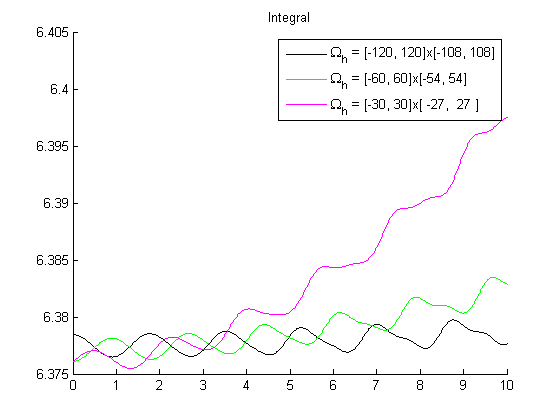
\includegraphics[width=\linewidth]{../amitans/figures/MassTaylor_120_60_30_ZB1_bt3_c045_h020_O(h^6).png}
	\end{minipage}	
	\begin{minipage}[b]{0.49\linewidth}
		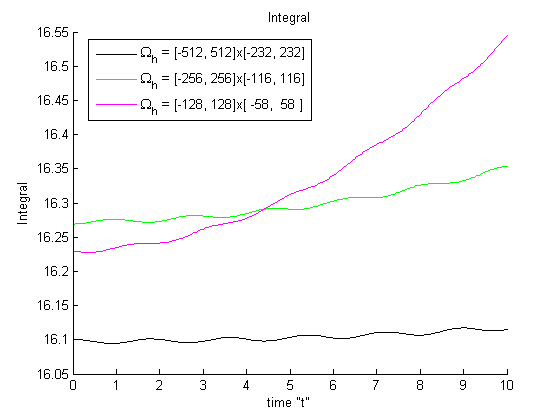
\includegraphics[width=\linewidth]{../amitans/figures/MassTaylor_512_256_128_ZB1_bt1_c090_h040_O(h^6).png}
		
	\end{minipage}
\end{center}
The Mass of the solution for approximation $O(|h|^6 + \tau^6)$ and $T = 10$ over three nested domains. Left panel is for Test 1 with $\beta=3$, $c = 0.45$ and right panel is for Test 2 with $\beta=1$, $c = 0.9$.
\end{frame}


\end{document}

